%! TeX program = xelatex
%! TeX TS-program = xelatex
%! TeX root = ProgramaciónEvolutiva.tex
%%%%%%%%%%%%%%%%%%%%%%%%%%%%%%%%%%%%%%%%%%%%%%%%%%%%%%%%%%%%%%%%%%%%%%%%
\definecolor{mypurple}{RGB}{104,020,108}
\setbeamercolor*{palette primary}{use=structure,fg=white,bg=mypurple}
\setbeamercolor{normal text}{fg=white, bg=black}
\setbeamercolor{tcolorbox text}{fg=white, bg=black}
\setbeamertemplate{navigation symbols}{}                              %
\newcommand{\colouredcircle}{%
  \tikz{\useasboundingbox (-0.2em,-0.32em) rectangle(0.2em,0.32em);
        \draw[ball color=PineGreen!7!Plum!90!Red,shading=ball,line width=0.03em] (0,0) circle(0.18em);}}
\newcommand{\colouredcircledis}{%
  \tikz{\useasboundingbox (-0.2em,-0.32em) rectangle(0.2em,0.32em);
        \draw[ball color=PineGreen!7!Plum!20!Black,shading=ball,line width=0.03em] (0,0) circle(0.18em);}}
\setbeamertemplate{itemize item}{\colouredcircle}
\setbeamercolor*{bibliography entry title}{fg=Cyan}
%%%%%%%%%%%%%%%%%%%%%%%%%%%%%%%%%%%%%%%%%%%%%%%%%%%%%%%%%%%%%%%%%%%%%%%%
\usepackage{tikzpagenodes}
\setbeamertemplate{background canvas}{%
  \begin{tikzpicture}[inner sep=0pt,remember picture,overlay]
    \node at (current page.center) {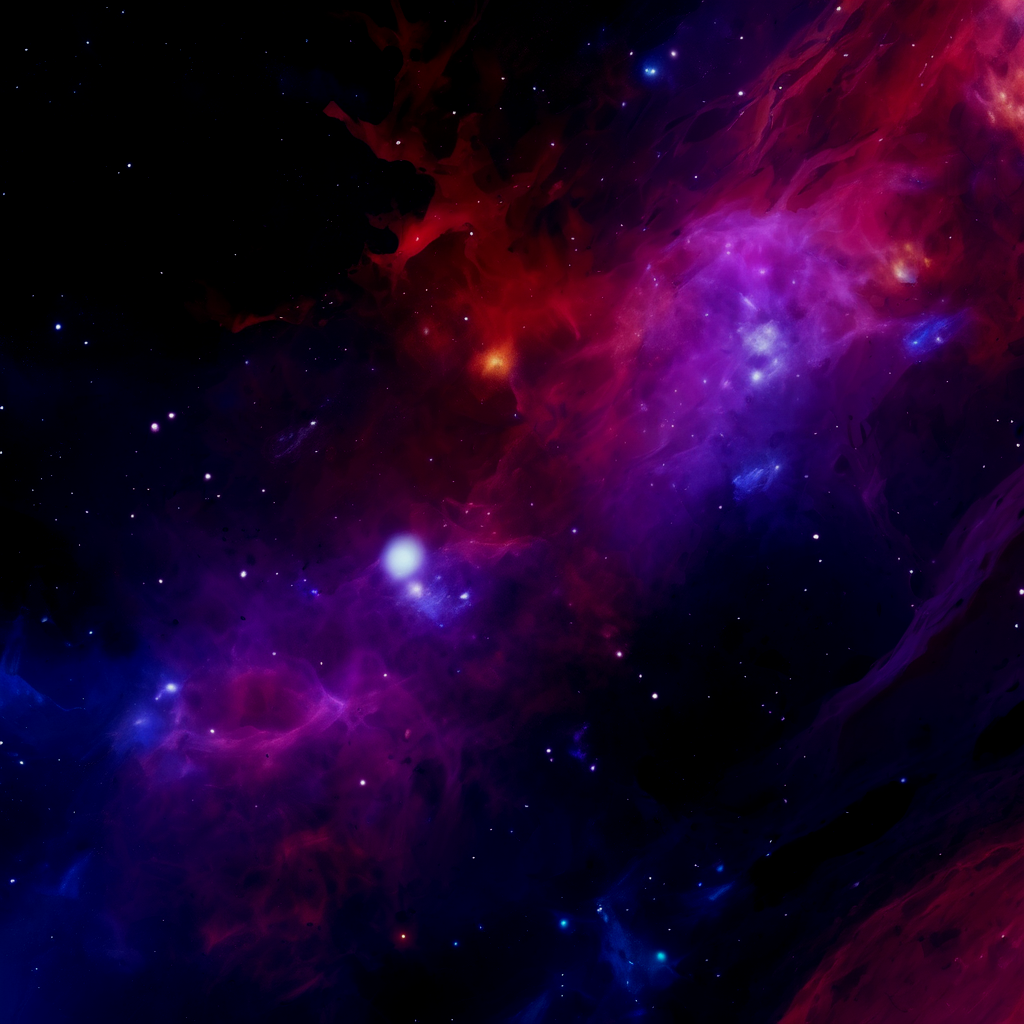
\includegraphics[height=\paperheight,width=\paperwidth]{fondo}};
  \end{tikzpicture}
}

\makeatletter
\newtcolorbox{blur}[1][]{%
  #1,
  enhanced,
  remember,
  frame hidden,
  interior hidden,
  fonttitle=\bfseries\centering, 
  fontupper=\rmfamily\selectfont,
  coltext=white,
  underlay={
    \begin{tcbclipframe}
      \begin{scope}[inner sep=0pt,remember picture,overlay]
        \fill[white] (current page.south west) rectangle (current page.north east);
        \node[opacity=1] at (current page.center) {
\includegraphics[height=\paperheight, width=\paperwidth]{blured}};
      \end{scope}
    \end{tcbclipframe}
   }
}
\makeatother
%%%%%%%%%%%%%%%%%%%%%%%%%%%%%%%%%%%%%%%%%%%%%%%%%%%%%%%%%%%%%%%%%%%%%%%%
\newcommand{\separador}[1]{
  \vskip-4pt
  \begin{center}
    \rule{0.9\linewidth}{#1}
  \end{center}
}

\lstset{
  basicstyle=\ttfamily,
  showstringspaces=false,
  breaklines=true
}

\newcommand{\transparencia}[1]{%
  \begin{frame}
    \begin{blur}
      #1
    \end{blur}
  \end{frame}
}

\bibliography{bibliografia}
\nocite{*}
